\subsection{Motion History}
\begin{table}[h!]
    \centering
    \begin{tabular}{ | l | c | c | c |}
        \hline
        Konfiguration & Beste & Unter 60 kB & Unter 28 kB \\\hline
        Ensemble-Methode & ExtraTrees & ExtraTrees & ExtraTrees \\\hline
        Maximalhöhe & 10 & 11 & 9 \\\hline
        Waldgröße & 16 & 10 & 6 \\\hline
        min\_samples\_leaf & 1 & 4 & 1 \\\hline
        Programmgröße in Bytes & 84200 & 57436 & 22804 \\\hline
        Genauigkeit Testmenge von Klisch & 68,8\% & 67,7\% & 62,5\% \\\hline
        Genauigkeit Gestentestmenge & 74,5\% & 69,6\% & 68,5\% \\\hline
        Genauigkeit Nullgestentestmenge & 68,3\% & 67,8\% & 67,6\% \\\hline
    \end{tabular}
    \caption{Beste Konfigurationen der Motion History.}
    \label{tab:motion_history}
\end{table}
\begin{figure}[h!]
    \centering
    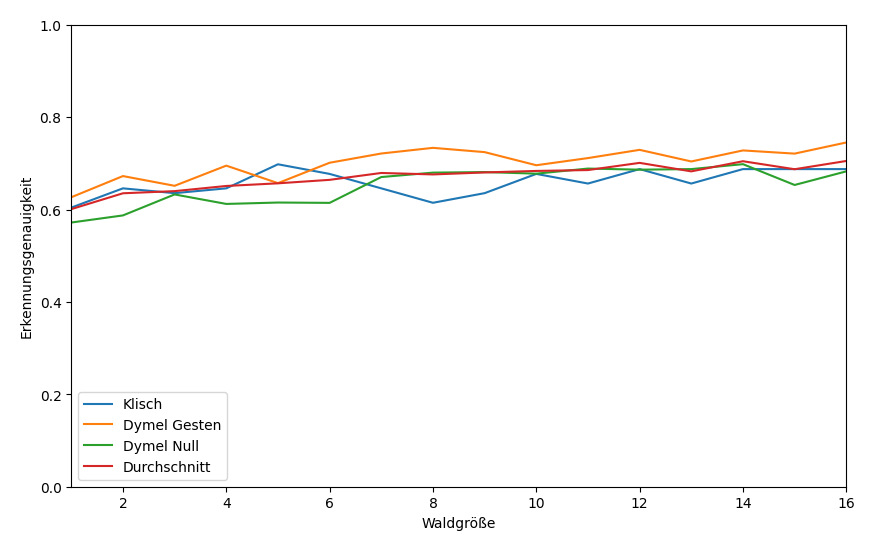
\includegraphics[width=\linewidth]{images/motion_history_acc_per_size.png}
    \caption{Die beste summierte Erkennungsgenauigkeit pro Waldgröße mit Motion History.}
    \label{fig:motion_history_per_forest_size}
\end{figure}
Die Featuremenge von Motion History beinhaltet für jeden Pixel einen Eintrag, die der Definition des Motion History Image folgen (siehe Formel \ref{formular:mhi}), wobei $\tau=100$ und $\delta=\frac{\tau}{\#Bilder}$ ist.
\newline
\newline
Die beste Konfiguration wurde mit der Ensemble-Methode \textit{ExtraTrees} gefunden (siehe Tabelle \ref{tab:helligkeitsverteilung}). Sie erzielt eine Erkennungsgenauigkeit von 68,8\% auf der Testmenge von Klisch,
74\% auf der Gestentestmenge und 69\% auf der Nullgestentestmenge. Im Vergleich zu der Helligkeitsverteilung wird mehr Programm-Speicher benötigt und die Gesamterkennungsganuigkeit ist 1,84\% geringer.
\newline
\newline
Wird die beste Konfiguration mit der \textit{Unter 28 kB} vergleichen, nimmt die Gesamterkennungsgenauigkeit nur um 4,3\% ab bei einer Reduktion der Programmgröße von 72,9\%. Im Vergleich zur Helligkeitsverteilung
gewinnt die Motion History mehr Gesamterkennungsgenauigkeit mit einer zunehmenden Waldgröße (siehe Abbildung \ref{fig:motion_history_per_forest_size}). Wenn der Suchraum nicht auf eine Waldgröße von 16 begrenzt wäre,
würde die beste Konfiguration vermutlich besser sein. Allerdings würde sich die Programmgröße signifikant erhöhen.
\newline
\newline
Die Motion History kann mit auschschließlich 8-Bit Integer implementiert werden und hat damit den geringsten WCET und Programmgröße pro Baum, weswegen die beste Konfiguration mit einer Waldgröße von 16 nicht deutlich
größer ist als die der Helligkeitsverteilung mit einer Waldgröße von 10.
